\documentclass[result.tex]{subfiles}

\begin{document}

    \section*{\centering Result}

    In this part of the report we will present the result that have been gathered from our two experiments on reward functions and state representations. It will be presented in the order aforementioned.

    \subsection*{Reward Experiment}

    In this section we will present the results given by the reward experiment. All the following plots will show the same results for the different algorithms. Note that the left column contains result using the board state representation and the right column is result for using the directional state. All the results have been averaged over 3 different experiments.

    \begin{figure}[ht]
        \centering
        \begin{subfigure}[b]{.35\linewidth}
            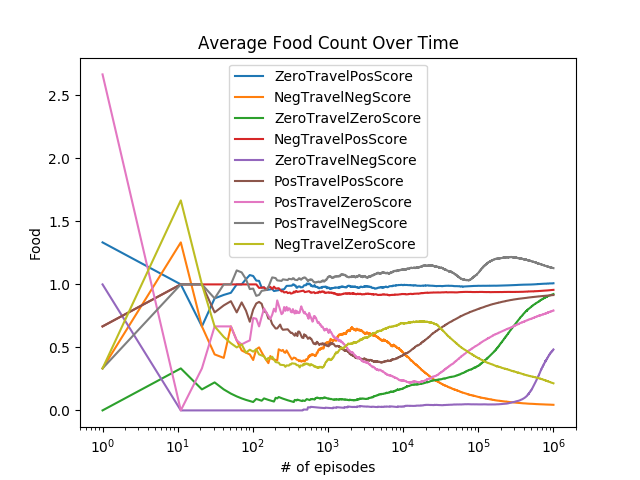
\includegraphics[width=\linewidth]{../images/qlearning/reward/234/board_state_average_food_count_over_time.png}
        \end{subfigure}
        \begin{subfigure}[b]{.35\linewidth}
            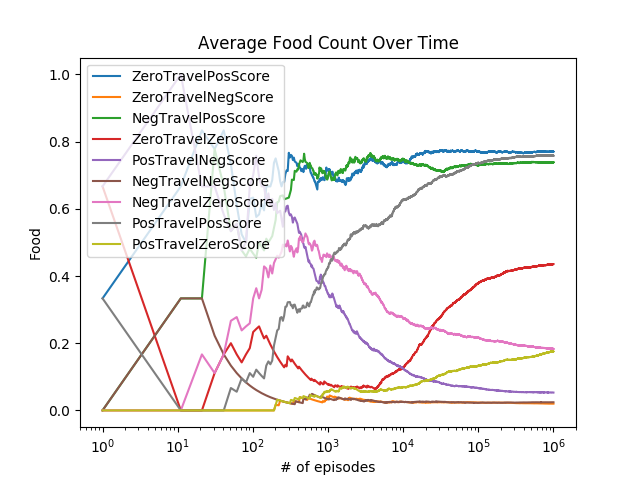
\includegraphics[width=\linewidth]{../images/qlearning/reward/234/directional_distance_state_average_food_count_over_time.png}
        \end{subfigure}

        \begin{subfigure}[b]{.35\linewidth}
            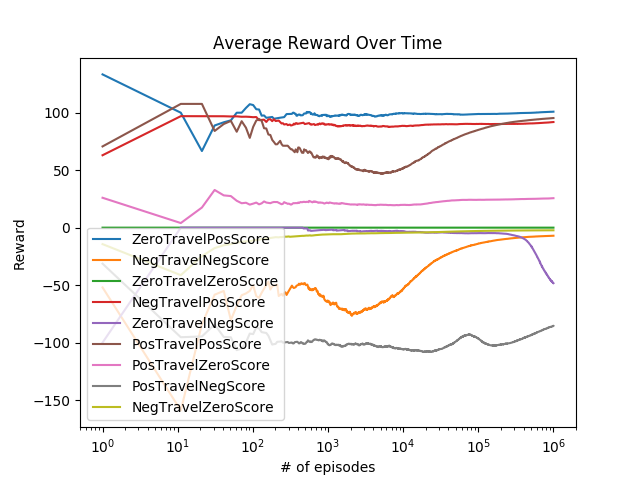
\includegraphics[width=\linewidth]{../images/qlearning/reward/234/board_state_average_reward_over_time.png}
        \end{subfigure}
        \begin{subfigure}[b]{.35\linewidth}
            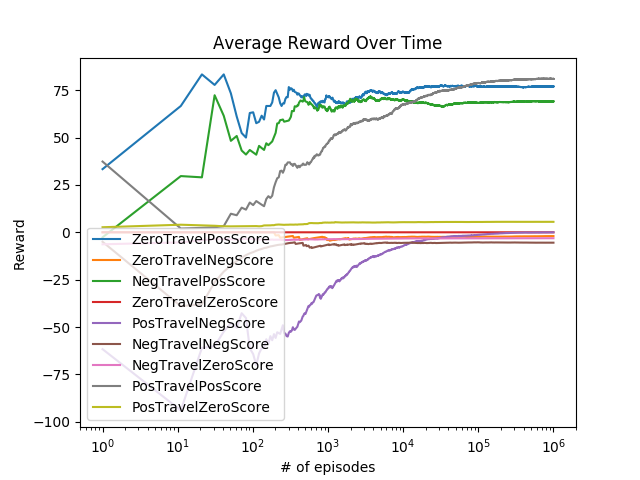
\includegraphics[width=\linewidth]{../images/qlearning/reward/234/directional_distance_state_average_reward_over_time.png}
        \end{subfigure}
        \caption{Results generated by Q-Learning.}
        \label{fig:reward_result_qlearning}
    \end{figure}

    \begin{figure}[ht]
        \centering
        \begin{subfigure}[b]{.35\linewidth}
            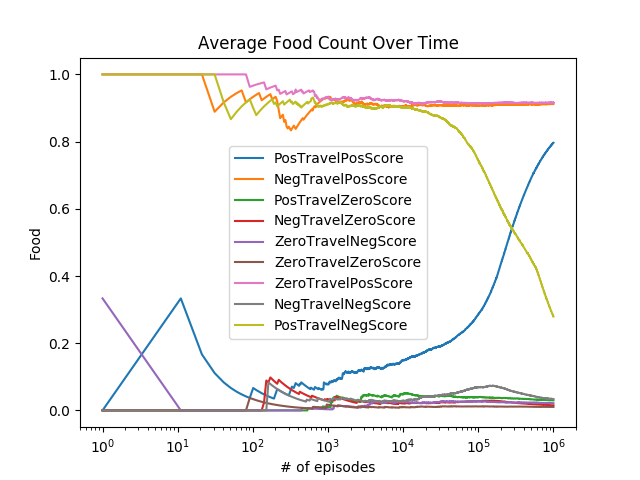
\includegraphics[width=\linewidth]{../images/sarsa/reward/234/board_state_average_food_count_over_time.png}
        \end{subfigure}
        \begin{subfigure}[b]{.35\linewidth}
            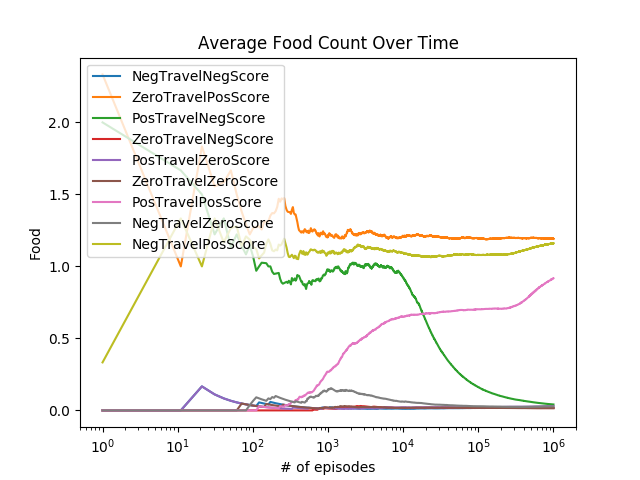
\includegraphics[width=\linewidth]{../images/sarsa/reward/234/directional_distance_state_average_food_count_over_time.png}
        \end{subfigure}

        \begin{subfigure}[b]{.35\linewidth}
            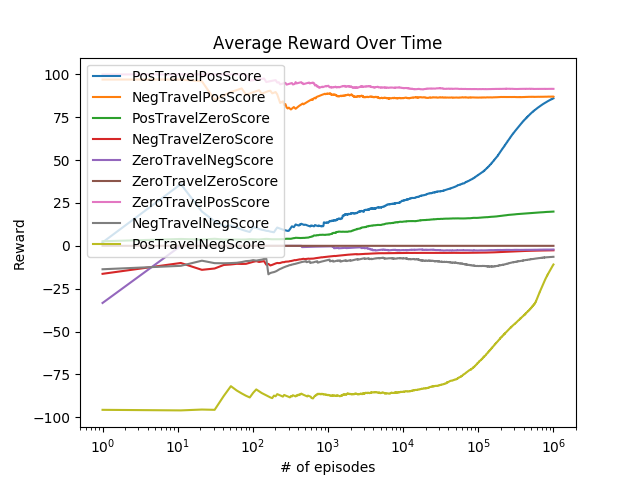
\includegraphics[width=\linewidth]{../images/sarsa/reward/234/board_state_average_reward_over_time.png}
        \end{subfigure}
        \begin{subfigure}[b]{.35\linewidth}
            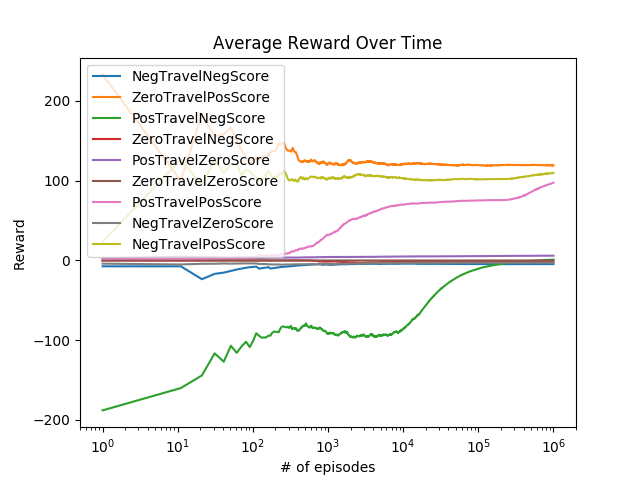
\includegraphics[width=\linewidth]{../images/sarsa/reward/234/directional_distance_state_average_reward_over_time.png}
        \end{subfigure}
        \caption{Results generated by Sarsa.}
        \label{fig:reward_result_sarsa}
    \end{figure}

    \newpage

    \begin{figure}[ht]
        \centering
        \begin{subfigure}[b]{.35\linewidth}
            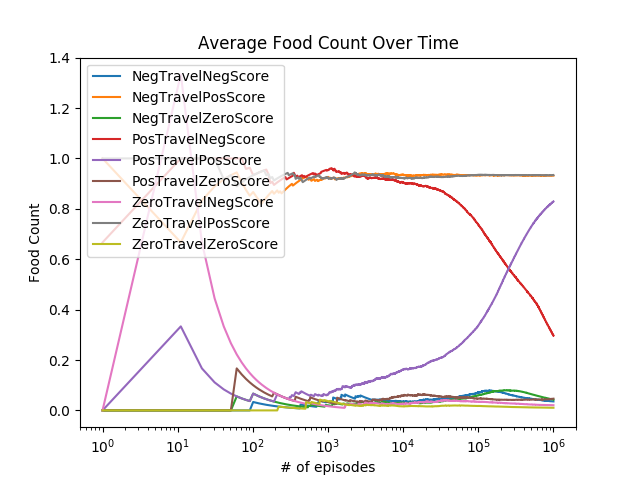
\includegraphics[width=\linewidth]{../images/expected_sarsa/reward/234/board_state_average_food_count_over_time.png}
        \end{subfigure}
        \begin{subfigure}[b]{.35\linewidth}
            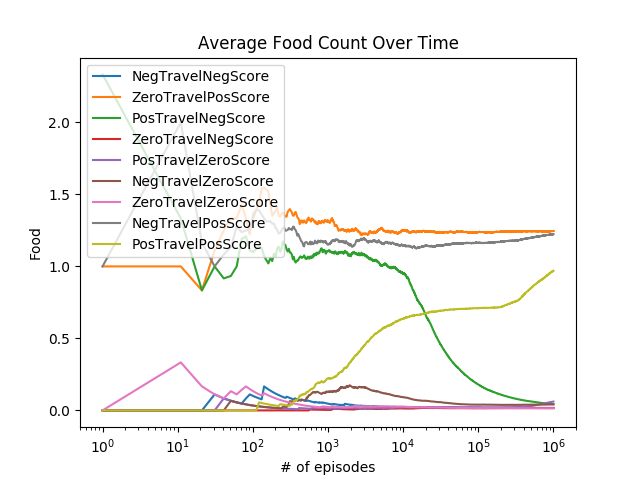
\includegraphics[width=\linewidth]{../images/expected_sarsa/reward/234/directional_distance_state_average_food_count_over_time.png}
        \end{subfigure}

        \begin{subfigure}[b]{.35\linewidth}
            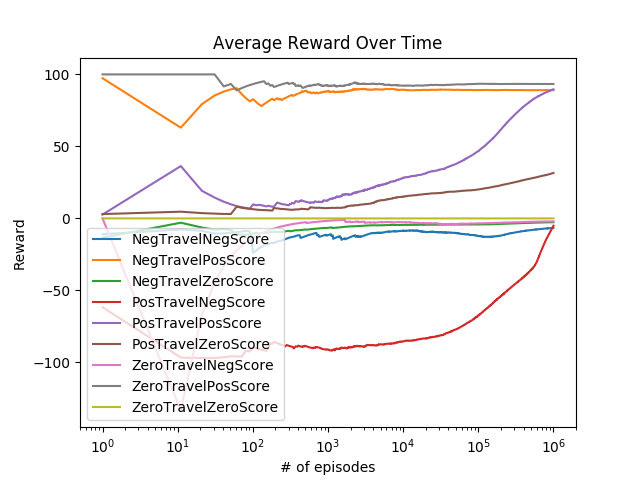
\includegraphics[width=\linewidth]{../images/expected_sarsa/reward/234/board_state_average_reward_over_time.png}
        \end{subfigure}
        \begin{subfigure}[b]{.35\linewidth}
            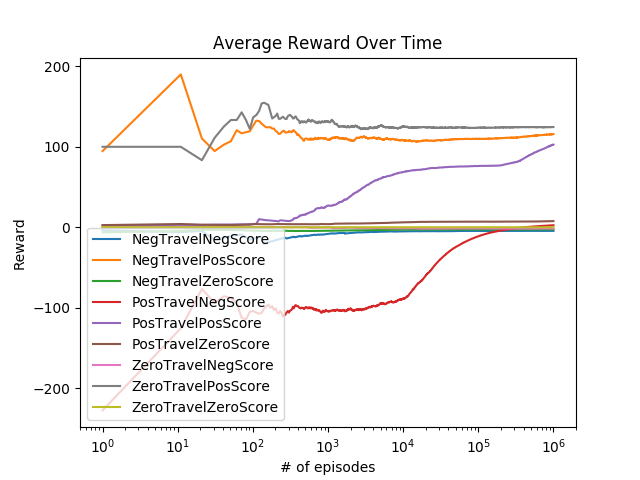
\includegraphics[width=\linewidth]{../images/expected_sarsa/reward/234/directional_distance_state_average_reward_over_time.png}
        \end{subfigure}
        \caption{Results generated by Expected Sarsa.}
        \label{fig:reward_result_expected_sarsa}
    \end{figure}

    The upper plots shows the average food the agent learns to eat on average which is the goal to maximize and the lower plots shows the average reward as a function of time for the different reward functions presented in the method.

    What we mean by \enquote{average over time} is that we take the average of all data points up to (inclusive) the time we are interested in, i.e., a moving average with an infinite tail. In our case time refers to the number of episodes we have trained the model.

    We also looked at the correlation between the curves in the column wise plots above shown in table \ref{tab:reward_food_corr}.

    \begin {table}[H]
        \begin{tabular}{c|c|c|}
            \cline{2-3}
            & \multicolumn{1}{ c| }{Avg. Correlation}
            & \multicolumn{1}{ c| }{Avg. Abs. Correlation} \\
            \cline{2-3}
            & \multicolumn{2}{ c| }{Q-Learning} \\
            \cline{1-3}
            \multicolumn{1}{ |c|  }{Board State}
            & 0.536742184842 & 0.945093533818 \\
            \cline{1-3}
            \multicolumn{1}{ |c|  }{Directional Distance State}
            & 0.49589001223 & 0.973537777401 \\
            \cline{1-3}
            & \multicolumn{2}{ c| }{Sarsa} \\
            \cline{1-3}
            \multicolumn{1}{ |c|  }{Board State}
            & 0.395990504669 & 0.978606301141 \\
            \cline{1-3}
            \multicolumn{1}{ |c|  }{Directional Distance State}
            & 0.521129553421 & 0.963340845075 \\
            \cline{1-3}
            & \multicolumn{2}{ c| }{Expected Sarsa} \\
            \cline{1-3}
            \multicolumn{1}{ |c|  }{Board State}
            & 0.457350122159 & 0.898156494946 \\
            \cline{1-3}
            \multicolumn{1}{ |c|  }{Directional Distance State}
            & 0.507751828694 & 0.968662042717 \\
            \cline{1-3}
        \end{tabular}
        \caption {Correlations between rewards and food counts.}
        \label{tab:reward_food_corr}
    \end{table}

    \newpage

    \subsubsection*{State Experiment}

    In this section we present the results from the state experiment. For each algorithm we have looked at the 16 states presented in the method and they are presented in three plots. Since the goal is to look at the objective of the problem we plot the average game score each state gets over 1 million episodes of training. Same as before we have averaged the result over 3 experiments.

    The first thing we looked at was augmenting the state representations with board dimensions and game score. Figure \ref{fig:info_augmentation_board_state} shows the results using the board representation and trained with Q-learning. We saw similar results for other states and algorithms.

    \begin{figure}[ht]
        \centering
        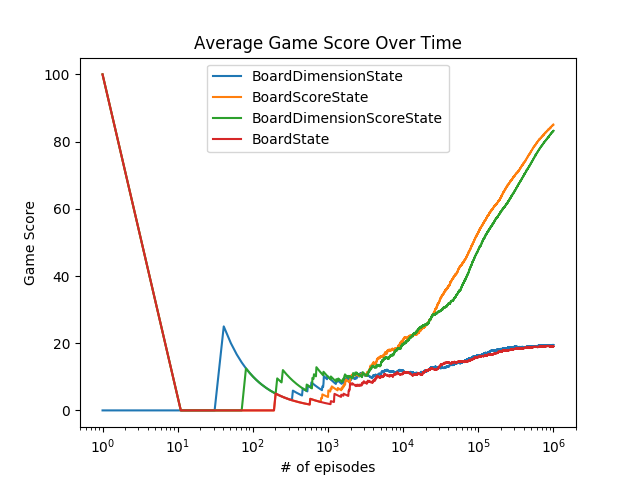
\includegraphics[width=\linewidth]{../images/qlearning/info_augmentation/123/board_state_average_game_score_over_time.png}
        \caption{Board state with different augmented information.}
        \label{fig:info_augmentation_board_state}
    \end{figure}

    \newpage

    We trained the models on a lot of different states as stated in the method and in figure \ref{fig:state_qlearning} shows the most promising states trained with Q-learning. We have included test performance in table \ref{table:state_qlearning} by averaging scores over 10000 episodes (games) and it also shows the performance of an agent that chooses action uniformly at random as a comparison of what we could expect from a terrible model.

    \begin{figure}[ht]
        \centering
        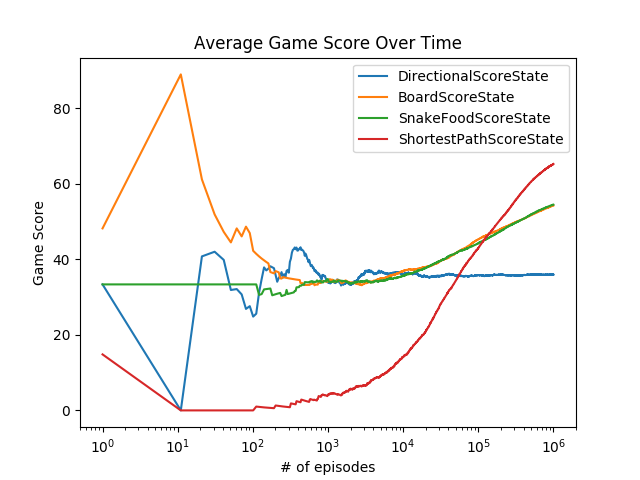
\includegraphics[width=\linewidth]{../images/qlearning/state/42/state_qlearning_average_game_score_over_time.png}
        \caption{Performance of state representations trained using Q-learning.}
        \label{fig:state_qlearning}
    \end{figure}

    \begin{table}[ht]
        \centering
        \begin{tabular}{ | l | l | l | }
            \hline
            State & Avg. Score & Std. Deviation \\ \hline
            ShortestPathScoreState & 129.50 & 51.11 \\ \hline
            BoardScoreState & 103.12 & 17.73 \\ \hline
            DirectionalScoreState & 66.12 & 64.328 \\ \hline
            SnakeFoodScoreState & 104.12 & 20.08 \\ \hline
            Random Agent & 20.13 & 46.47 \\
            \hline
        \end{tabular}
        \caption{Test performance over 10000 episodes.}
        \label{table:state_qlearning}
    \end{table}

    \newpage

    Similar results as previously are shown in figure \ref{fig:state_sarsa} and table \ref{table:state_sarsa} but trained with Sarsa. We have not included any results for Expected Sarsa since its performance and behavior was very similar to Sarsa. The appendix at the end includes more results on other states that was less promising in terms of game score performance.

    \begin{figure}[ht]
        \centering
        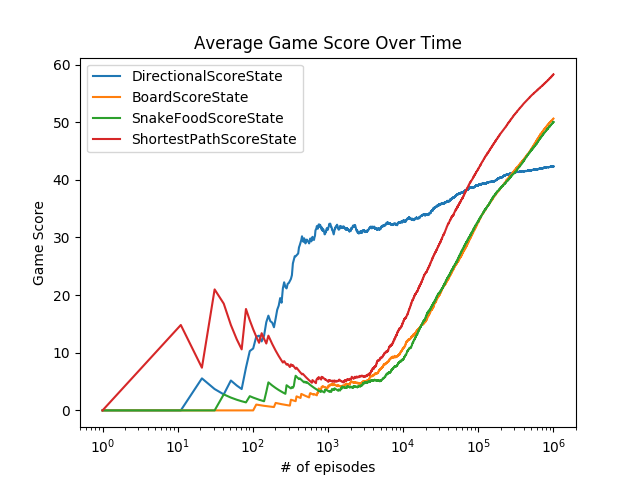
\includegraphics[width=\linewidth]{../images/sarsa/state/42/state_sarsa_average_game_score_over_time.png}
        \caption{Performance of state representations trained using Sarsa.}
        \label{fig:state_sarsa}
    \end{figure}

    \begin{table}[ht]
        \centering
        \begin{tabular}{ | l | l | l | }
            \hline
            State & Avg. Score & Std. Deviation \\ \hline
            ShortestPathScoreState & 118.59 & 38.95 \\ \hline
            BoardScoreState & 101.02 & 10.05 \\ \hline
            DirectionalScoreState & 72.16 & 71.60 \\ \hline
            SnakeFoodScoreState & 101.02 & 10.05 \\
            \hline
        \end{tabular}
        \caption{Test performance over 10000 episodes.}
        \label{table:state_sarsa}
    \end{table}

\end{document}
